% ==========================================================
% Póster académico A1 horizontal · 3 columnas · VERSIÓN EN INGLÉS
% Maestría en Inteligencia Artificial Aplicada · Equipo 1
% Basado en poster_plantilla.tex (encabezado, colores, fuentes y tamaños de la plantilla).
% Compilación: latexmk -pdf poster_proyecto_en.tex (figuras *_en.png de generar_figuras.py)
% ==========================================================
\documentclass[10pt]{article}

\usepackage{iftex}
\usepackage[a1paper,landscape,margin=1.5cm]{geometry}
\usepackage[english]{babel}
\usepackage{xcolor}
\usepackage{graphicx}
\usepackage{tikz}
\usetikzlibrary{arrows.meta,positioning,calc}
\usepackage[most]{tcolorbox}
\usepackage{enumitem}
\usepackage{booktabs}
\usepackage{colortbl}
\usepackage{microtype}

% ---------------------- TIPOGRAFÍA -------------------------
\ifTUTeX
  \usepackage{fontspec}
  \IfFontExistsTF{Instrument Serif}%
    {\newfontfamily\serif{Instrument Serif}}%
    {\newfontfamily\serif{TeX Gyre Pagella}}
\else
  \usepackage[utf8]{inputenc}
  \usepackage[T1]{fontenc}
  \usepackage{lmodern}
  \usepackage[scaled=0.95]{helvet}
  \newcommand{\serif}{\fontfamily{bch}\selectfont}
\fi

\pagestyle{empty}
\setlength{\parindent}{0pt}
\setlength{\parskip}{0.4em}

% ---------------------- PALETA -----------------------------
\definecolor{olive}{HTML}{9AA542}
\definecolor{olivedark}{HTML}{1B2208}
\definecolor{olivelink}{HTML}{6B7A1F}
\definecolor{olivesoft}{HTML}{E4E8C7}
\definecolor{ink}{HTML}{1A1A10}
\definecolor{muted}{HTML}{6B6B5E}
\definecolor{pagebg}{HTML}{FFFFFF}
% Grises y azul pizarra de las figuras (generar_figuras.py)
\definecolor{graysoft}{HTML}{E6E4DE}
\definecolor{slatedark}{HTML}{1F2A36}
% Figura 2: rampa salvia (verde azulado) de claro a oscuro; distinguible con daltonismo (ΔE OKLab >= 16)
\definecolor{salvia1}{HTML}{A8C5BD}
\definecolor{salvia2}{HTML}{5F958A}
\definecolor{salvia3}{HTML}{2E5E56}

\pagecolor{pagebg}
\color{ink}

% ---------------------- DATOS DEL PÓSTER -------------------
\newcommand{\programa}{Master in Applied Artificial Intelligence}
\newcommand{\tituloA}{Self-supervised learning with Contrastive Predictive Coding}
\newcommand{\tituloB}{to recognize manual material handling activities}
\newcommand{\autores}{Isaura Yutsil Flores Escamilla\quad Paola Alejandra León Guarneros\quad Dylan Ulises Quiroz Hernández}
\newcommand{\asesor}{Dr. Gerardo Jesús Camacho González}
\newcommand{\fecha}{November 2026}

\newcommand{\logoizq}{
\includegraphics[height=3.3cm]{logo.jpeg}}
\newcommand{\logoder}{
\includegraphics[height=3.3cm]{logo_der.png}}

% ---------------------- ESTILOS ----------------------------
\newcommand{\seccion}[1]{%
  \begin{tcolorbox}[colback=olive,colframe=olive,arc=0pt,
    boxrule=0pt,left=8pt,top=3pt,bottom=4pt,width=\linewidth]
    {\serif\color{white}\fontsize{30}{36}\selectfont #1}
  \end{tcolorbox}\vspace{-0.3em}}

\newcommand{\cuerpo}{\fontsize{24}{31}\selectfont}
\newcommand{\pie}[1]{{\sffamily\fontsize{18}{22}\selectfont\color{muted}#1}}

\newcommand{\circulo}[1]{%
  \tikz\node[circle,fill=graysoft,minimum size=6cm,align=center,
    text width=5cm,text=slatedark,
    font=\sffamily\bfseries\fontsize{19}{23}\selectfont]{#1};}

% Tarjeta de cifra: \cifra{ancho}{valor}{descripción}
\newcommand{\cifra}[3]{%
  \begin{minipage}[t]{#1}
  \begin{tcolorbox}[colback=graysoft,colframe=graysoft,arc=4pt,boxrule=0pt,
    width=\linewidth,left=6pt,right=6pt,top=6pt,bottom=6pt,halign=center,valign=center,height=4.6cm]
    {\serif\fontsize{48}{52}\selectfont\color{slatedark}#2}\\[0.15em]
    {\sffamily\fontsize{18}{22}\selectfont\color{ink}#3}
  \end{tcolorbox}
  \end{minipage}}

% Actividad: \act{código}{nombre}
\newcommand{\act}[2]{%
  \tikz\node[draw=olive,line width=1.5pt,rounded corners=4pt,fill=white,minimum width=5.55cm,
    minimum height=2.1cm,align=center,inner sep=4pt]
    {{\sffamily\bfseries\fontsize{24}{26}\selectfont\color{olivelink}#1}\\[2pt]
     {\sffamily\fontsize{16}{19}\selectfont\color{ink}#2}};}

\newlength{\hdrh}\setlength{\hdrh}{9cm}
\newlength{\colh}
\setlength{\colh}{\dimexpr\textheight-\hdrh-6cm\relax}

% ======================================================
\begin{document}

% ---------------------- ENCABEZADO ------------------------
\noindent\parbox[t][\hdrh][c]{\linewidth}{%
\begin{minipage}[c]{0.145\linewidth}
  \raggedright\logoizq
\end{minipage}%
\begin{minipage}[c]{0.71\linewidth}
  \centering
  {\serif\fontsize{58}{65}\selectfont\color{olivedark}%
   \tituloA\\\tituloB\par}
  \vspace{0.5em}
  {\sffamily\bfseries\fontsize{30}{36}\selectfont\color{olivelink}\programa\par}
  \vspace{0.3em}
  {\fontsize{26}{32}\selectfont\color{ink}\autores\par}
  {\fontsize{22}{28}\selectfont\color{muted}Advisor: \asesor\ \textperiodcentered\ \fecha\par}
\end{minipage}%
\begin{minipage}[c]{0.145\linewidth}
  \raggedleft\logoder
\end{minipage}}

\vspace{0.4cm}
{\color{olive}\rule{\linewidth}{2.5pt}}
\vspace{0.6cm}

% ---------------------- COLUMNAS --------------------------
\noindent
\begin{minipage}[t][\colh][s]{0.30\linewidth}\cuerpo\vspace{0pt}
% ===== COLUMNA IZQUIERDA: problema y datos =====

\seccion{Why recognize activities?}
Manual material handling is one of the tasks most associated with \textbf{musculoskeletal injuries}. To detect harmful movements, we first need to know \textbf{what} the worker is doing and \textbf{when}.

\begin{center}
\act{N}{Neutral posture}\hspace{0.15cm}\act{LF}{Lift from floor}\hspace{0.15cm}\act{K}{Hold the load}\hspace{0.15cm}\act{W}{Walk with load}\\[0.2cm]
\act{LT}{Lift from table}\hspace{0.15cm}\act{PT}{Place on table}\hspace{0.15cm}\act{PF}{Place on floor}
\end{center}

\begin{minipage}[c]{0.40\linewidth}
  \centering
  
\begin{tikzpicture}
    \fill[olivesoft] (0,0) arc (180:0:4.5 and 4.5) -- (6,0) arc (0:180:3 and 3) -- cycle;
    \node[font=\serif\fontsize{64}{68}\selectfont,text=olivedark] at (4.5,1.1) {600};
  \end{tikzpicture}
\end{minipage}\hfill
\begin{minipage}[c]{0.58\linewidth}
  segments marked \textbf{by hand} for each recorded person. Annotation is slow and costly.
\end{minipage}

\vspace{0.3em}
\begin{tcolorbox}[colback=olivesoft,colframe=olive,boxrule=2pt,arc=4pt,left=10pt,right=10pt]
\textbf{Question:} can a model pretrained \emph{without labels} match a supervised one on new people, and beat it with \textbf{few labels}?
\end{tcolorbox}

\vfill
\seccion{Data and evaluation}
14 people · 37 trials · loads from 2 to 12~kg · suit with 17 inertial sensors and electromyography (sEMG).
\begin{center}
  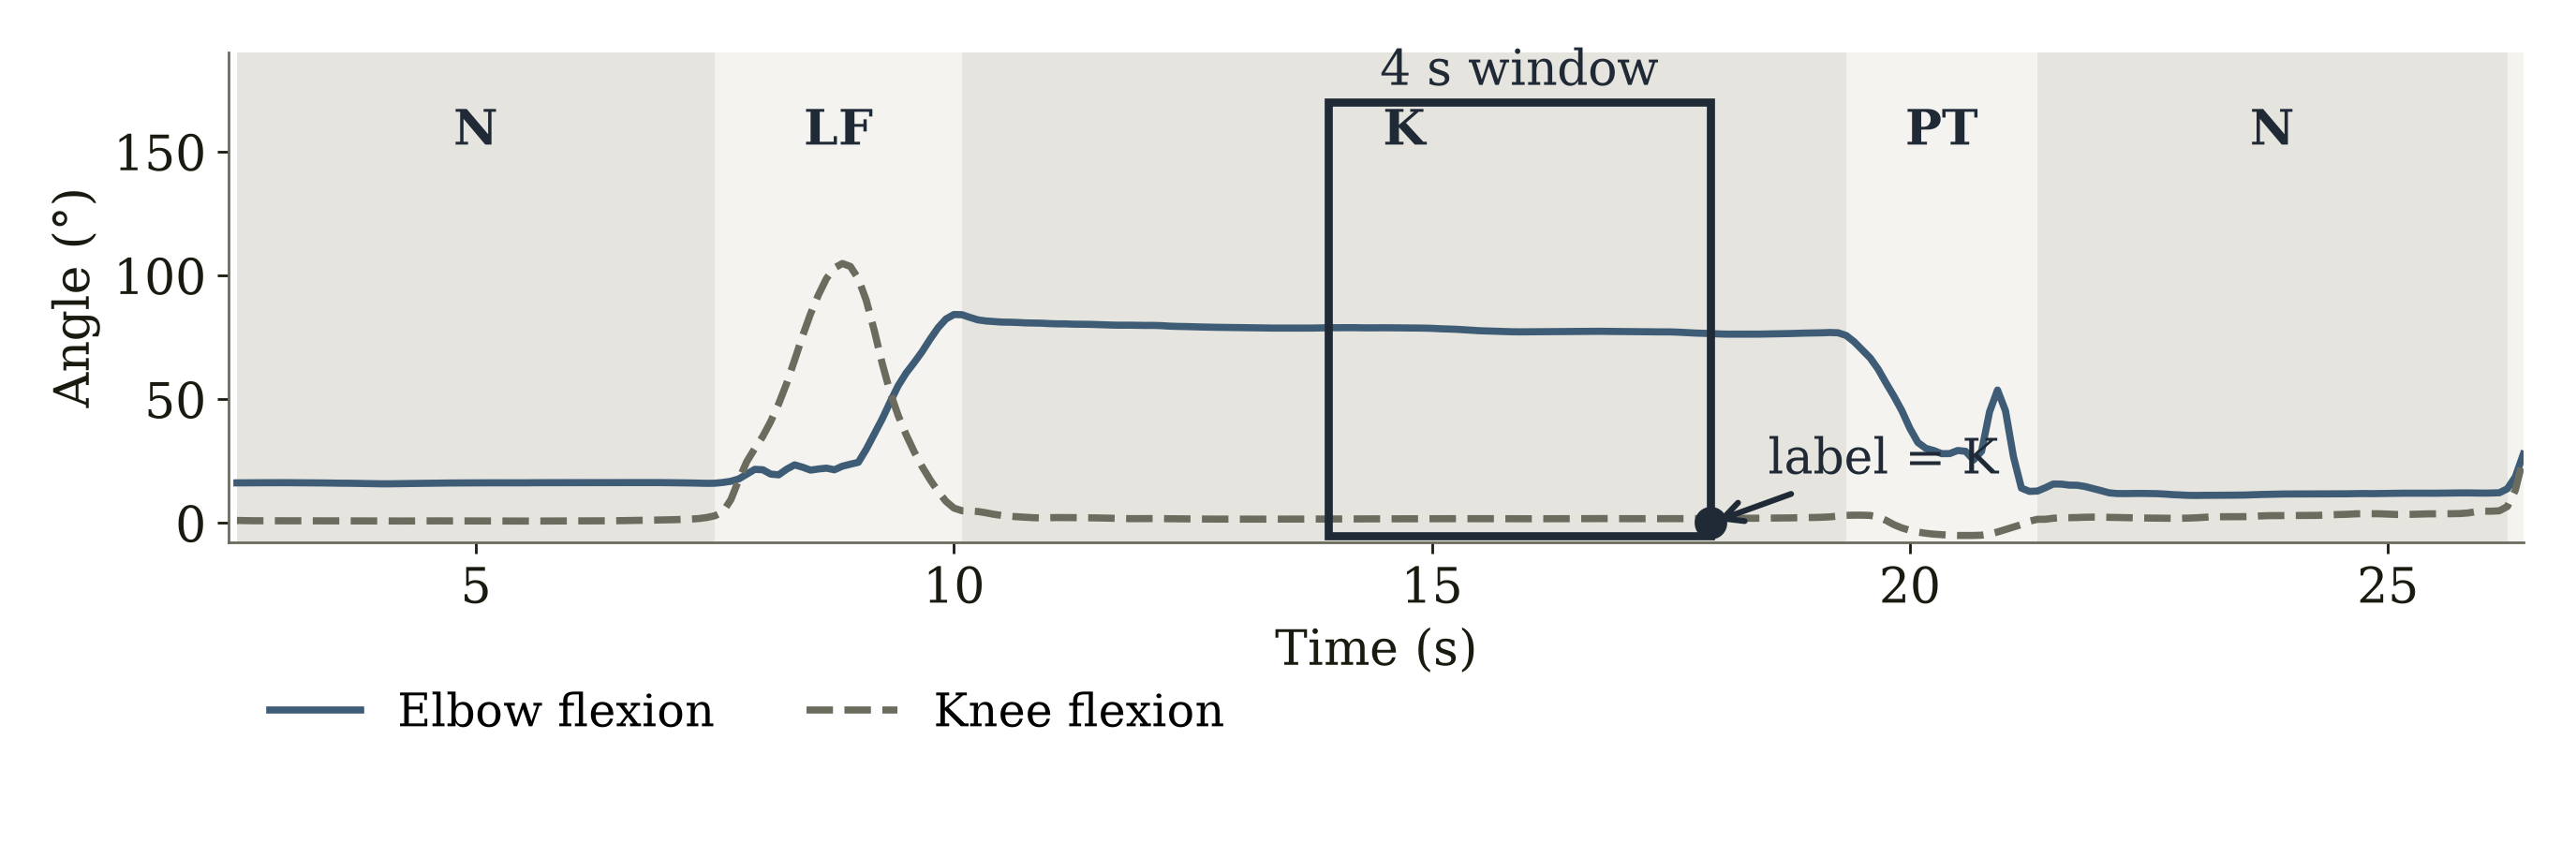
\includegraphics[width=\linewidth]{fig_ventana_en.png}\\[2pt]
  \pie{Figure 1. Each 4 s window is labeled with the activity at its last instant.}
\end{center}
Always on \textbf{new people}: 12 leave-one-subject-out rounds, plus 2 people held out for the final test.

\vfill
\seccion{From muscle to movement}
\begin{center}
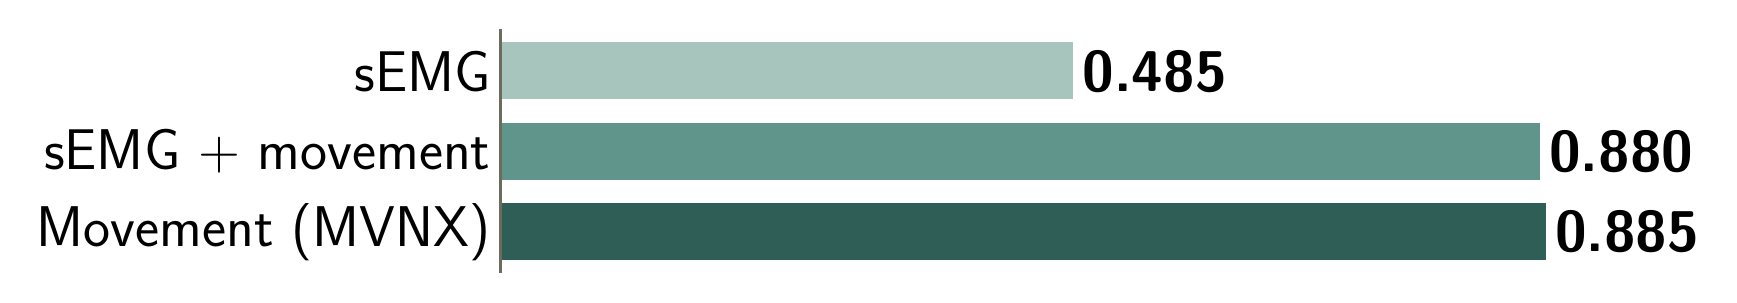
\begin{tikzpicture}[x=15cm,y=0.85cm]
  \foreach \y/\lab/\v/\c in {2.4/sEMG/0.485/salvia1, 1.2/sEMG + movement/0.880/salvia2, 0/Movement (MVNX)/0.885/salvia3}{
    \fill[\c] (0,\y) rectangle (\v,\y+0.85);
    \node[anchor=east,font=\sffamily\fontsize{20}{24}\selectfont] at (0,\y+0.42) {\lab};
    \node[anchor=west,font=\sffamily\bfseries\fontsize{20}{24}\selectfont] at (\v,\y+0.42) {\v};
  }
  \draw[muted,line width=1pt] (0,-0.2) -- (0,3.45);
\end{tikzpicture}\\[2pt]
\pie{Figure 2. Macro F1 with each source: only movement tells floor from table.}
\end{center}

\end{minipage}\hfill
\begin{minipage}[t][\colh][s]{0.37\linewidth}\cuerpo\vspace{0pt}
% ===== COLUMNA CENTRAL: modelo y hallazgo principal =====

\seccion{The model: CPC with a GRU network}
\begin{center}
\begin{tikzpicture}[
  font=\sffamily\fontsize{20}{24}\selectfont,
  box/.style={draw=olivelink,line width=2pt,rounded corners=4pt,align=center,minimum height=2.6cm,inner sep=5pt,fill=white},
  pre/.style={box,fill=olivesoft},
  aux/.style={box,dashed,draw=muted,text=muted},
  head/.style={box,fill=olive,text=white,draw=olive},
  arr/.style={-{Stealth[length=6mm]},line width=3pt,color=olivelink}]
  \node[box,text width=4.3cm] (x) {4 s window\\ 10 variables};
  \node[pre,right=0.9cm of x,text width=4.3cm] (enc) {Causal\\ encoder};
  \node[pre,right=0.9cm of enc,text width=3.2cm] (gru) {GRU};
  \node[aux,right=1.4cm of gru,yshift=1.75cm,text width=8.6cm,minimum height=2.3cm] (pred) {\textbf{Phase 1 · no labels}\\ predicts movement\\ up to 1 s ahead};
  \node[head,right=1.4cm of gru,yshift=-1.75cm,text width=8.6cm,minimum height=2.3cm] (cab) {\textbf{Phase 2 · with labels}\\ linear head $\to$ 7 activities};
  \draw[arr] (x) -- (enc);
  \draw[arr] (enc) -- (gru);
  \draw[arr,muted] (gru.east) -- ++(0.7,0) |- (pred.west);
  \draw[arr] (gru.east) -- ++(0.7,0) |- (cab.west);
\end{tikzpicture}\\[4pt]
\pie{Figure 3. It learns without labels and is then fine-tuned with few (725k parameters, causal).}
\end{center}

\vfill
\seccion{11 of 17 sensors are enough}
\begin{minipage}[c]{0.36\linewidth}
\centering
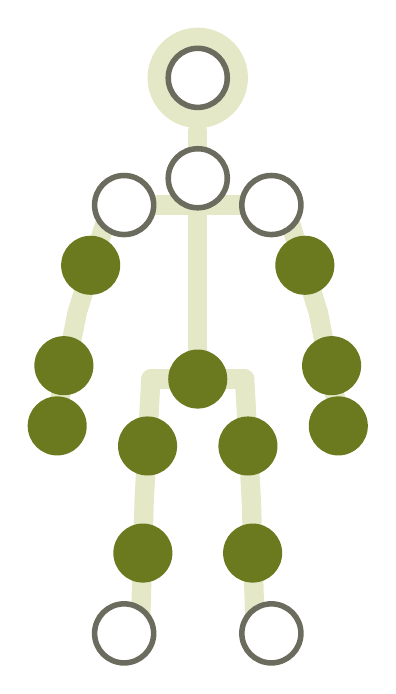
\begin{tikzpicture}[scale=0.85,
  keep/.style={circle,fill=olivelink,minimum size=0.75cm,inner sep=0pt},
  drop/.style={circle,draw=muted,line width=2pt,fill=white,minimum size=0.75cm,inner sep=0pt},
  bone/.style={line width=7pt,color=olivesoft,line cap=round}]
  % skeleton
  \draw[bone] (0,7.3) -- (0,3.6);
  \draw[bone] (-1.3,6.2) -- (1.3,6.2);
  \draw[bone] (-1.3,6.2) -- (-1.8,4.6) -- (-2.1,3.1);
  \draw[bone] (1.3,6.2) -- (1.8,4.6) -- (2.1,3.1);
  \draw[bone] (-0.7,3.6) -- (0.7,3.6);
  \draw[bone] (-0.7,3.6) -- (-0.8,1.8) -- (-0.85,0.1);
  \draw[bone] (0.7,3.6) -- (0.8,1.8) -- (0.85,0.1);
  \fill[olivesoft] (0,8.1) circle (0.75);
  % removed sensors
  \node[drop] at (0,8.1) {}; \node[drop] at (0,6.6) {};
  \node[drop] at (-1.1,6.2) {}; \node[drop] at (1.1,6.2) {};
  \node[drop] at (-1.1,-0.2) {}; \node[drop] at (1.1,-0.2) {};
  % kept sensors
  \node[keep] at (0,3.6) {};
  \foreach \s in {-1,1}{
    \node[keep] at (\s*1.6,5.3) {}; \node[keep] at (\s*2.0,3.8) {}; \node[keep] at (\s*2.1,2.9) {};
    \node[keep] at (\s*0.75,2.6) {}; \node[keep] at (\s*0.82,1.0) {};
  }
\end{tikzpicture}
\end{minipage}\hfill
\begin{minipage}[c]{0.60\linewidth}
\tikz\node[circle,fill=olivelink,minimum size=0.75cm]{}; kept (11): pelvis, upper arms, forearms, hands, thighs and lower legs.\par
\tikz\node[circle,draw=muted,line width=2pt,minimum size=0.75cm]{}; removed (6): head, upper trunk, shoulders and feet.\par
\vspace{0.3em}
F1 of \textbf{0.873} vs.\ 0.878 with all 17: \textbf{no significant difference}.
\end{minipage}

\vfill
\seccion{Main finding: with few labels, CPC wins}
\begin{center}
  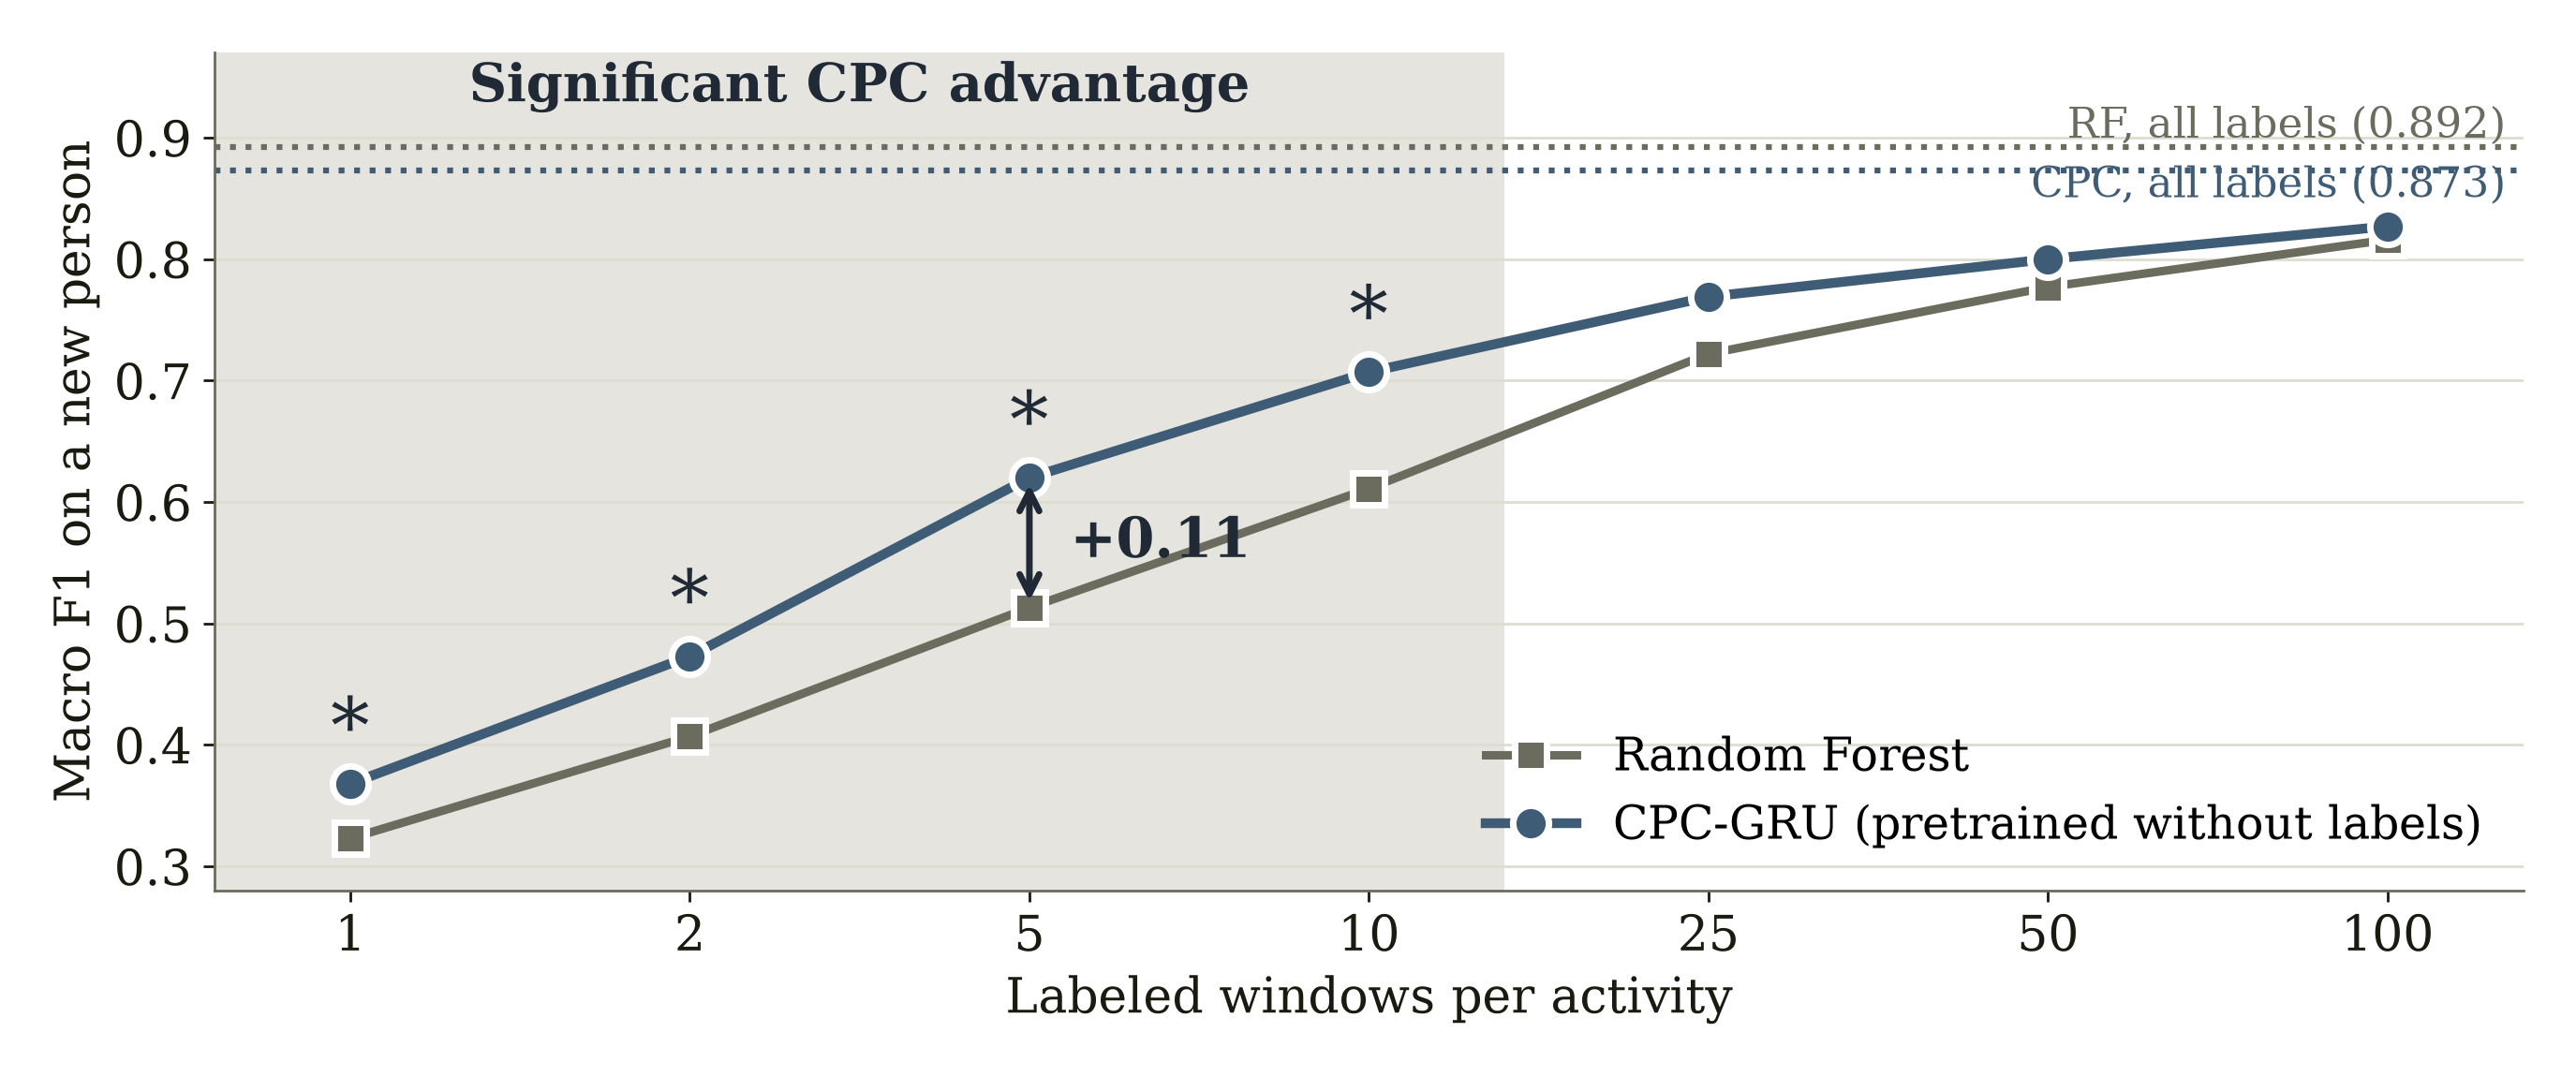
\includegraphics[width=\linewidth]{fig_pocas_en.png}\\[2pt]
  \pie{Figure 4. Macro F1 on a new person (* $p < 0.05$, Wilcoxon with Holm correction).}
\end{center}
\noindent
\cifra{0.32\linewidth}{+0.11}{F1 over Random Forest\\ with 5 windows per activity}\hfill
\cifra{0.32\linewidth}{2.2$\times$}{fewer labels for\\ the same performance}\hfill
\cifra{0.32\linewidth}{11--12}{of 12 people improve\\ with $\le 10$ windows}

\end{minipage}\hfill
\begin{minipage}[t][\colh][s]{0.30\linewidth}\cuerpo\vspace{0pt}
% ===== COLUMNA DERECHA: desempeño, conclusiones y aplicación =====

\seccion{How well does it work?}

\begin{center}
\pie{Table 1. Macro F1 with all labels.}

\vspace{0.3em}
\fontsize{20}{26}\selectfont
\renewcommand{\arraystretch}{1.35}
\arrayrulecolor{olivedark}
\begin{tabular}{lcc}
  \toprule
  \textbf{Model} & \textbf{New people} & \textbf{Final test} \\
  \midrule
  Random Forest (10 var.) & 0.892 & 0.885 · 0.906 \\
  \textbf{CPC-GRU (10 var.)} & \textbf{0.873} & \textbf{0.884 · 0.898} \\
  BiLSTM (Bassani et al., 2025) & 0.903$^{*}$ & --- \\
  \bottomrule
\end{tabular}\\[3pt]
\pie{$^{*}$ A single person and a different protocol; in a replication, CPC-GRU scored 0.910.}
\end{center}
With all labels, CPC comes \textbf{close} to the supervised model. Errors lie at the boundaries between activities; floor and table are rarely confused ($\le 4$\,\%).

\vfill
\seccion{Key conclusions}
\begin{center}
  \circulo{Movement\\outperforms\\sEMG}\hspace{0.2cm}
  \circulo{11 sensors\\are enough}\hspace{0.2cm}
  \circulo{With few\\labels,\\CPC wins}
\end{center}
CPC pays off when there is \textbf{plenty of recorded movement and few annotations}: the case of a new person, task or environment.

\vfill
\seccion{Toward application}
\begin{center}
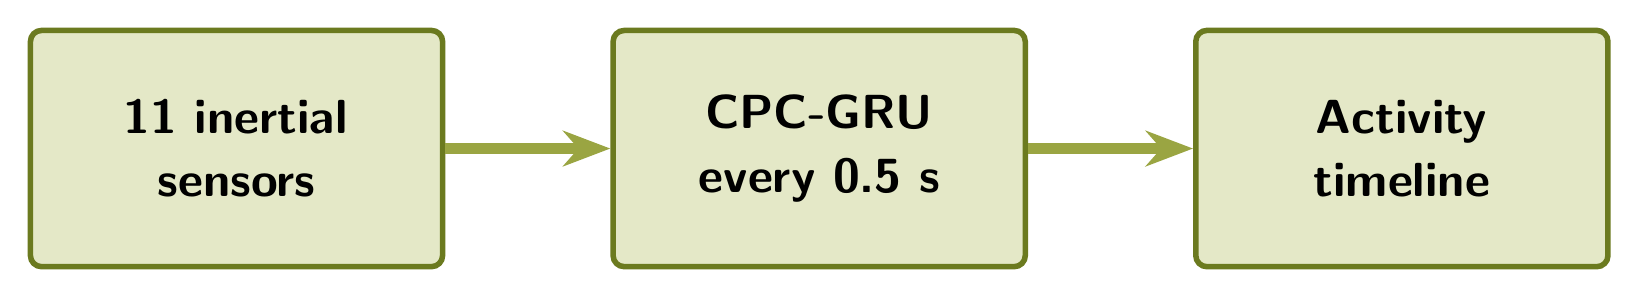
\begin{tikzpicture}[
  paso/.style={draw=olivelink,line width=2pt,rounded corners=4pt,fill=olivesoft,align=center,
    font=\sffamily\bfseries\fontsize{19}{23}\selectfont,text width=5cm,minimum height=3cm},
  arr/.style={-{Stealth[length=6mm]},line width=4pt,color=olive}]
  \node[paso] (a) at (0,0) {11 inertial\\ sensors};
  \node[paso] (b) at (7.4,0) {CPC-GRU\\ every 0.5 s};
  \node[paso] (c) at (14.8,0) {Activity\\ timeline};
  \draw[arr] (a.east) -- (b.west);
  \draw[arr] (b.east) -- (c.west);
\end{tikzpicture}
\end{center}
Next step: validate with workers and a real 11-sensor kit, and move from activities to \textbf{harmful movements}.

\vfill
\seccion{References}
{\fontsize{18}{23}\selectfont
\begin{itemize}[leftmargin=1.2em,itemsep=0.2em]
  \item Bassani, G., Avizzano, C. A., \& Filippeschi, A. (2025). Deep learning algorithms for human activity recognition in manual material handling tasks. \emph{Sensors, 25}(21), 6705.
  \item Bassani, G., Filippeschi, A., \& Avizzano, C. A. (2021). \emph{Manual material handling dataset for biomechanical and ergonomics analysis} [Data set]. Zenodo.
  \item Haresamudram, H., Essa, I., \& Plötz, T. (2021). Contrastive predictive coding for human activity recognition. \emph{Proc.\ ACM IMWUT, 5}(2), 1--26.
  \item van den Oord, A., Li, Y., \& Vinyals, O. (2018). \emph{Representation learning with contrastive predictive coding}. arXiv:1807.03748.
\end{itemize}}

\end{minipage}

\vfill
% ---------------------- DECLARACIÓN DE IA ------------------
{\color{olive}\rule{\linewidth}{2.5pt}}
\vspace{0.3cm}

\noindent
{\fontsize{18}{23}\selectfont\color{ink}
{\serif\color{olivedark}\fontsize{22}{28}\selectfont Statement on the use of artificial intelligence.}
Claude Code (Anthropic, 2026) was used to format this poster.
The authors are solely responsible for the content.\par}

\end{document}
